\documentclass{standalone}
\usepackage{tikz}
\usepackage{amsmath}
\usepackage{xcolor}
\usetikzlibrary{arrows.meta, decorations.pathreplacing, backgrounds, positioning, calc}
% Define custom colors
\definecolor{softyellow}{HTML}{F2D648}
\definecolor{dustyblue}{HTML}{9EB9D4}
\definecolor{berkeleyblue}{RGB}{0, 50, 98}
\definecolor{berkeleygold}{RGB}{253, 181, 21}

\begin{document}

\begin{center}\vspace{-0.55cm}
\begin{tabular}{@{}c@{\hspace{1cm}}c@{\hspace{1cm}}c@{}}
  % Row 1: Titles
  \textcolor{berkeleyblue}{\textbf{Twistronics}} & 
  \textcolor{berkeleyblue}{\textbf{Artificial Lattices}} & 
  \textcolor{berkeleyblue}{\textbf{Magnetic Fields}} \\[0.3cm]
  
  % Row 2: Figures
  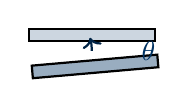
\begin{tikzpicture}[scale=0.8]
    \draw[thick, fill=berkeleyblue!20] (-1,-0.2) rectangle (1,0);
    \draw[thick, fill=berkeleyblue!40, rotate=5] (-1,-0.7) rectangle (1,-0.5);
    \draw[->, thick, berkeleyblue!70!black] (0,-0.35) arc[start angle=0, end angle=15, radius=0.8];
    \node at (0.9,-0.35) {\textcolor{berkeleyblue}{$\theta$}};
  \end{tikzpicture}
  &
  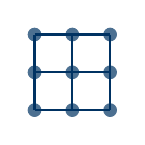
\begin{tikzpicture}[scale=0.8]
    \foreach \x in {-0.6,0,0.6} {
      \foreach \y in {0,0.6,1.2} {
        \filldraw[berkeleyblue!70] (\x,-\y) circle (0.1);
      }}
    \foreach \y in {0,0.6,1.2} {
      \draw[thick, berkeleyblue] (-0.6,-\y) -- (0.6,-\y);
    }
    \foreach \x in {-0.6,0,0.6} {
      \draw[thick, berkeleyblue] (\x,0) -- (\x,-1.2);
    }
  \end{tikzpicture}
  &
  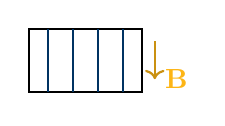
\begin{tikzpicture}[scale=0.8]
    \draw[thick] (-0.9,0) rectangle (0.9,-1);
    \foreach \x in {-0.6,-0.2,0.2,0.6} {
      \draw[berkeleyblue, thick] (\x,0) -- (\x,-1);
    }
    \draw[thick, ->, berkeleygold!80!black] (1.1,-0.2) -- (1.1,-0.8) node[right] {\textcolor{berkeleygold}{$\mathbf{B}$}};
  \end{tikzpicture}
  \\[0.5cm]
  
  % Row 3: Bullet Points
  \begin{minipage}[t]{0.28\textwidth}
    \footnotesize
    \begin{itemize}
      \item Precise layer stacking
      \item Magic angles ($\sim$1.1°)
      \item Complex fabrication
    \end{itemize}
  \end{minipage}
  &
  \begin{minipage}[t]{0.28\textwidth}
    \footnotesize
    \begin{itemize}
      \item Engineered geometries
      \item Optical/photonic systems
      \item Limited tunability
    \end{itemize}
  \end{minipage}
  &
  \begin{minipage}[t]{0.28\textwidth}
    \footnotesize
    \begin{itemize}
      \item Landau quantization
      \item Requires extreme fields
      \item Not practical for devices
    \end{itemize}
  \end{minipage}
\end{tabular}
\end{center}
\end{document}
